\documentclass[12pt]{amsart}


\usepackage{times}
\usepackage[margin=.9in]{geometry}
\usepackage{amsmath,amssymb,multicol,graphicx,framed,ifthen,color,xcolor,stmaryrd,enumitem,colonequals,bbm}


\usepackage[outline]{contour}
\contourlength{.4pt}
\contournumber{10}
\newcommand{\Bold}[1]{\contour{black}{#1}}


\definecolor{chianti}{rgb}{0.6,0,0}
\definecolor{meretale}{rgb}{0,0,.6}
\definecolor{leaf}{rgb}{0,.35,0}
\newcommand{\Q}{\mathbb{Q}}
\newcommand{\N}{\mathbb{N}}
\newcommand{\Z}{\mathbb{Z}}
\newcommand{\R}{\mathbb{R}}
\newcommand{\C}{\mathbb{C}}
\newcommand{\e}{\varepsilon}
\newcommand{\m}{\mathfrak{m}}
\newcommand{\p}{\mathfrak{p}}
\newcommand{\ord}{\mathrm{ord}}
\newcommand{\1}{\mathbbm{1}}
\newcommand{\cZ}{\mathcal{Z}}

\newcommand{\inv}{^{-1}}
\newcommand{\dabs}[1]{\left| #1 \right|}
\newcommand{\ds}{\displaystyle}
\newcommand{\solution}[1]{\ifthenelse {\equal{\displaysol}{1}} {\begin{framed}{\color{meretale}\noindent #1}\end{framed}} { \ }}
\newcommand{\showsol}[1]{\def\displaysol{#1}}
\newcommand{\rsa}{\rightsquigarrow}

\newcommand\itemA{\stepcounter{enumi}\item[{\Bold{(\theenumi)}}]}
\newcommand\itemB{\stepcounter{enumi}\item[(\theenumi)]}
\newcommand\itemC{\stepcounter{enumi}\item[{\it{(\theenumi)}}]}
\newcommand\itema{\stepcounter{enumii}\item[{\Bold{(\theenumii)}}]}
\newcommand\itemb{\stepcounter{enumii}\item[(\theenumii)]}
\newcommand\itemc{\stepcounter{enumii}\item[{\it{(\theenumii)}}]}
\newcommand\itemai{\stepcounter{enumiii}\item[{\Bold{(\theenumiii)}}]}
\newcommand\itembi{\stepcounter{enumiii}\item[(\theenumiii)]}
\newcommand\itemci{\stepcounter{enumiii}\item[{\it{(\theenumiii)}}]}
\newcommand\ceq{\colonequals}

\DeclareMathOperator{\res}{res}
\setlength\parindent{0pt}
%\usepackage{times}

%\addtolength{\textwidth}{100pt}
%\addtolength{\evensidemargin}{-45pt}
%\addtolength{\oddsidemargin}{-60pt}

\pagestyle{empty}
%\begin{document}\begin{itemize}

%\thispagestyle{empty}

\usepackage[hang,flushmargin]{footmisc}


\begin{document}
\showsol{0}
	
	\thispagestyle{empty}
	
	\section*{\S4.16: Nullstellensatz}	

\begin{framed}

\noindent \textsc{Definition:} Let $K$ be a field and $R=K[X_1,\dots,X_n]$. For a set of polynomials $S\subseteq R$, we define the \textbf{zero-set} of \textbf{solution set} of $S$ to be
\[ \cZ(S) \ceq \{ (a_1,\dots,a_n)\in K^n \ | \ F(a_1,\dots,a_n)=0 \ \text{for all} \ F\in S\}.\]

\

\noindent \textsc{Nullstellensatz:} Let $K$ be an algebraically closed field, and $R=K[X_1,\dots,X_n]$ be a polynomial ring. Let $I\subseteq R$ be an ideal. Then $\cZ(I)=\varnothing$ if and only if $I=R$ is the unit ideal. 

Put another way, a set $S$ of multivariate polynomials has a common zero unless there is a ``certificate of infeasibility'' consisting of $f_1,\dots,f_t\in S$ and $r_1,\dots,r_t\in R$ such that $\sum_i r_i s_i = 1$.

\

\noindent \textsc{Proposition:} Let $K$ be an algebraically closed field, and $R=K[X_1,\dots,X_n]$ be a polynomial ring. Every maximal ideal of $R$ is of the form $\m_\alpha = (X_1-a_1,\dots,X_n-a_n)$ for some point $\alpha=(a_1\dots,a_n)\in K^n$.

\end{framed}

 
\begin{enumerate}
\itemA Draw the ``real parts'' of $\cZ(X^2+Y^2-1)$ and of $\cZ(XY,XZ)$.

\solution{
\begin{center}
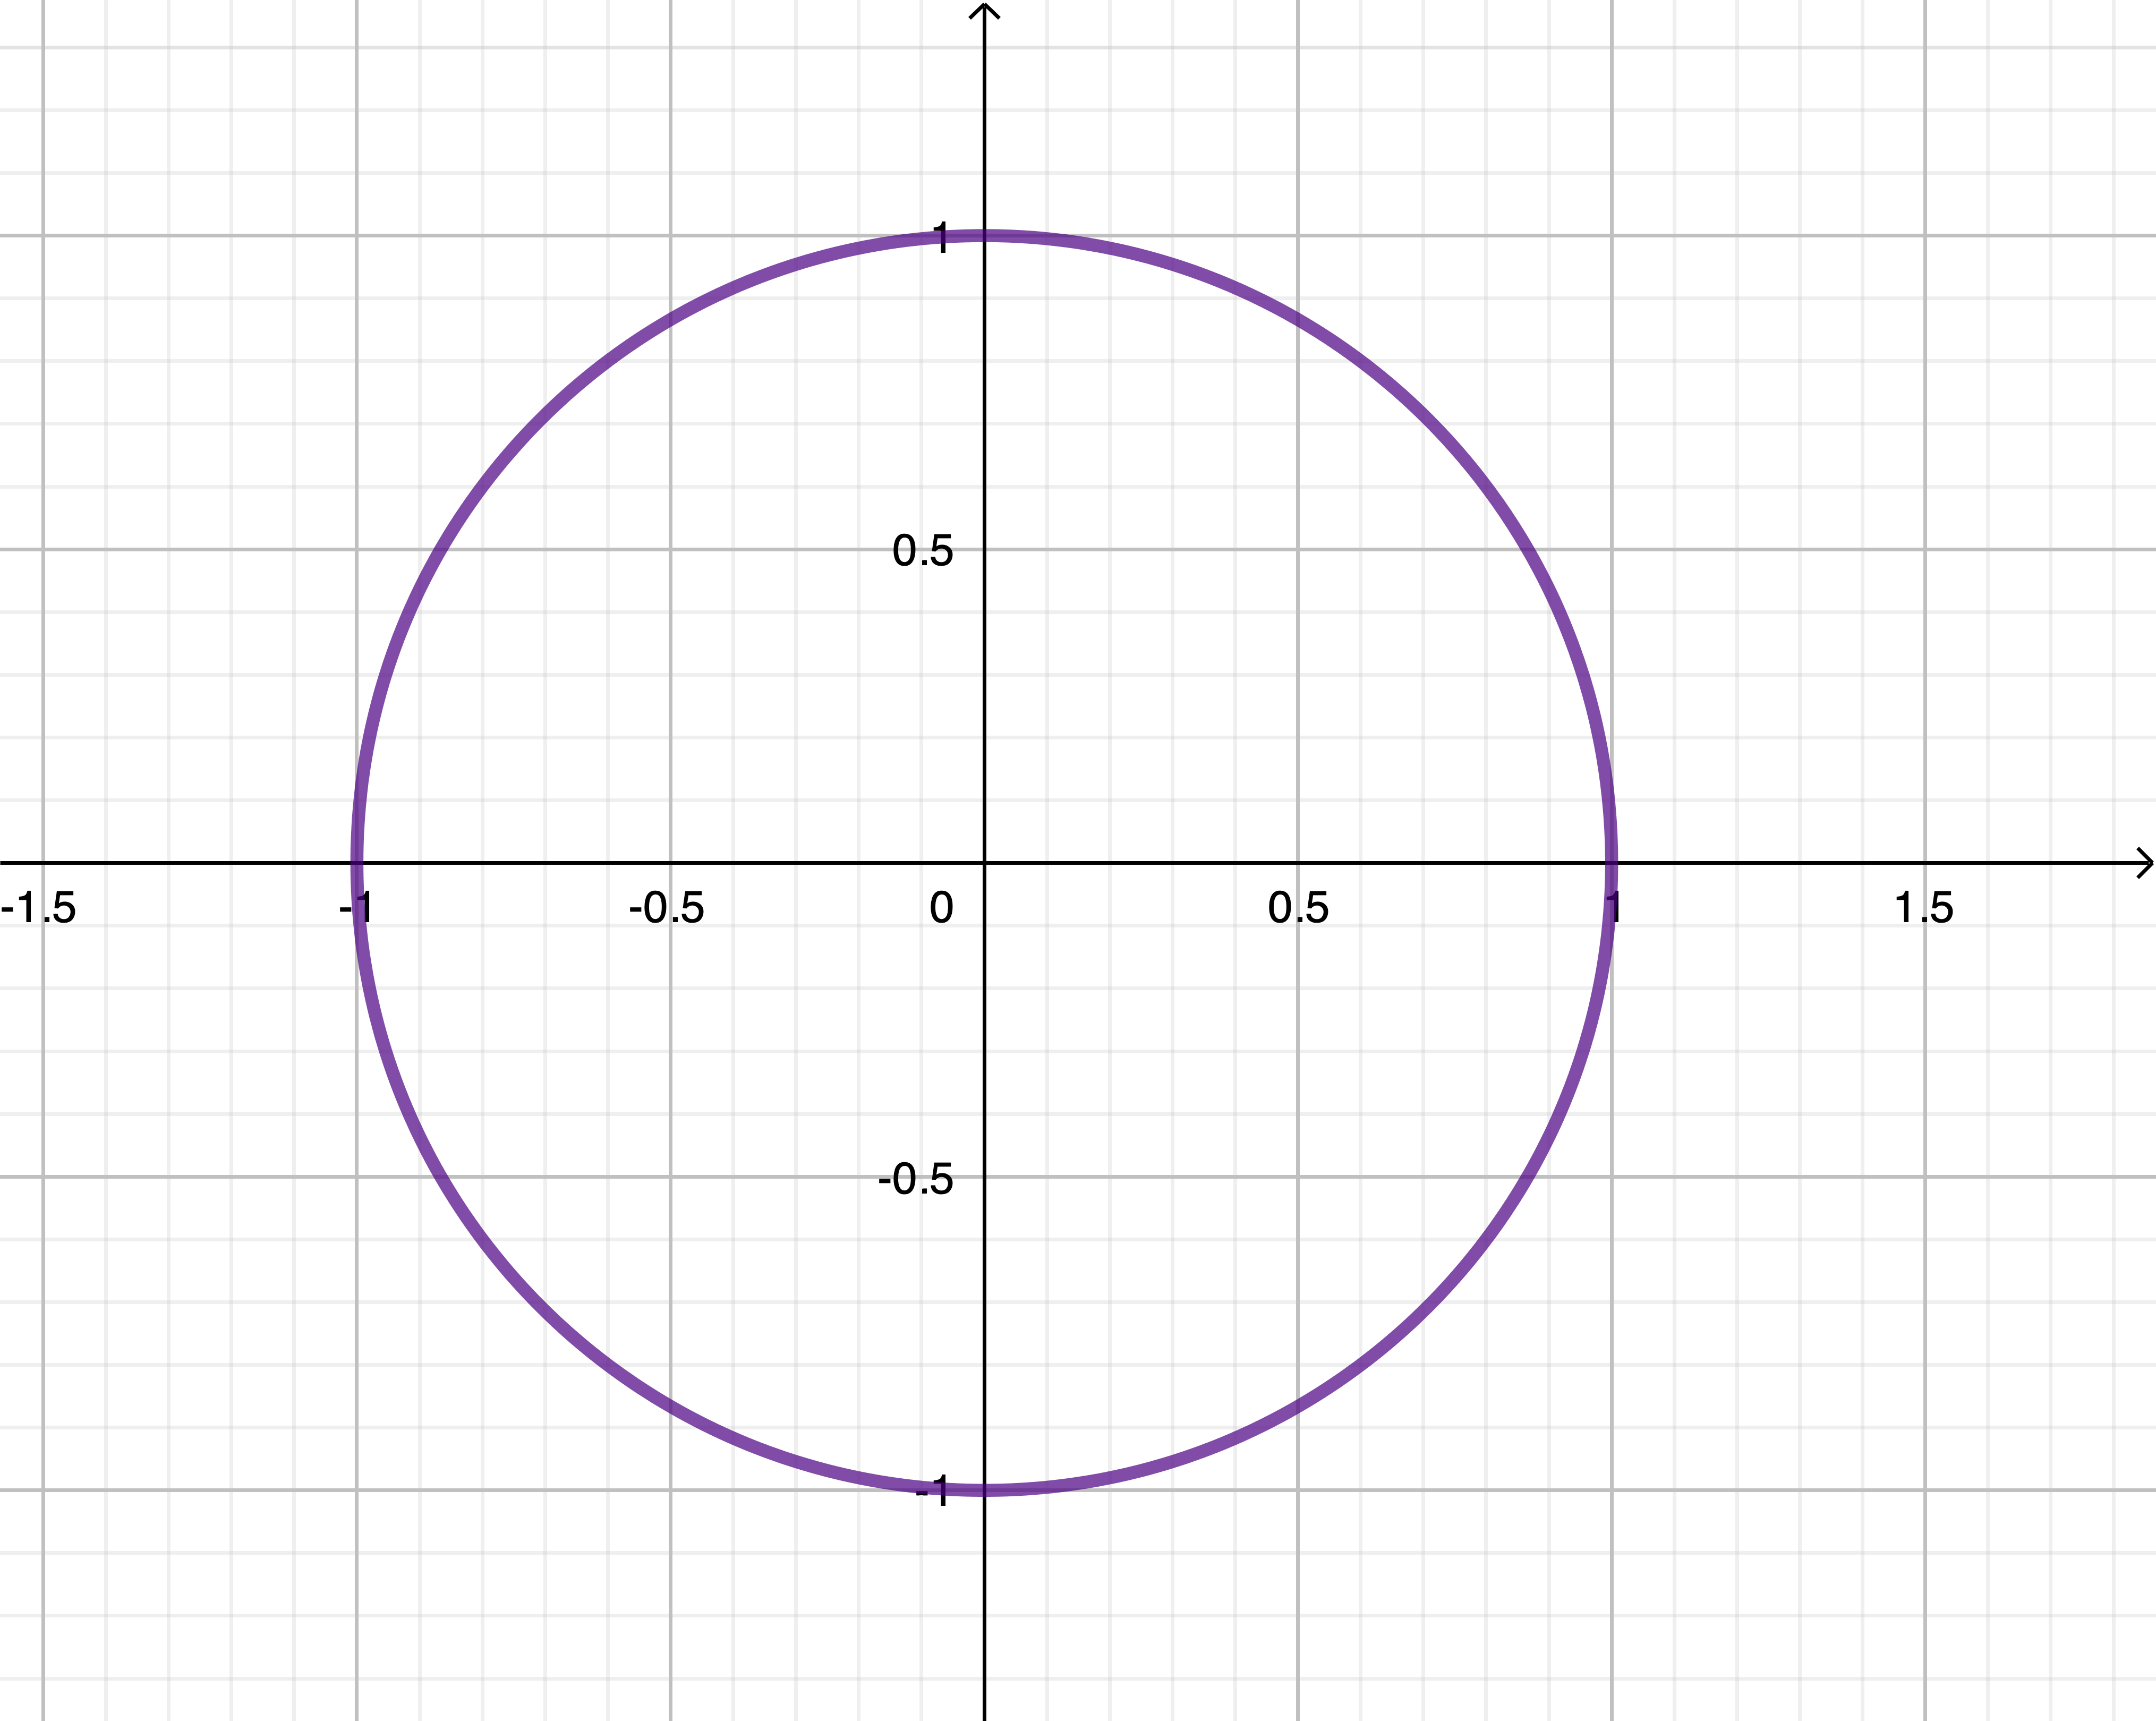
\includegraphics[scale=.15]{N1}\qquad
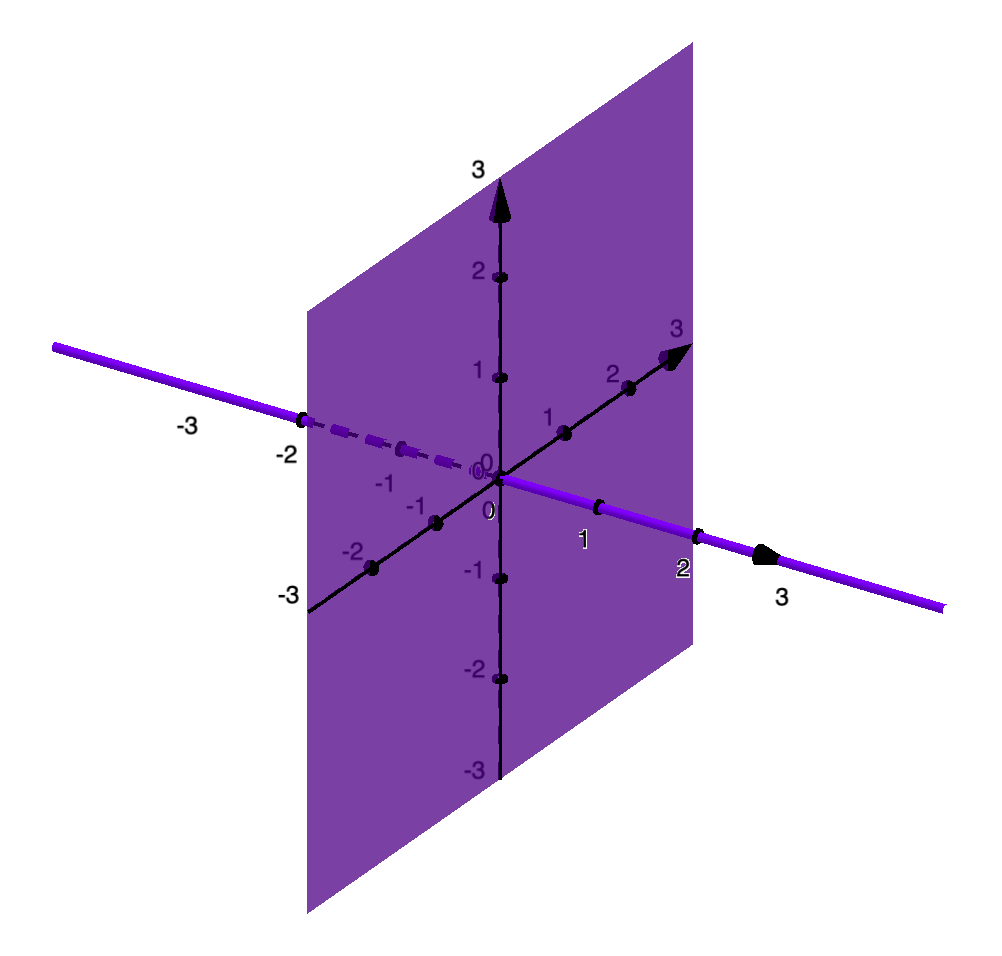
\includegraphics[scale=.5]{N2}
\end{center}
}

\itemA Explain why the Nullstellensatz is definitely false if $K$ is assumed to \emph{not} be algebraically closed.

\solution{
To not be algebraically closed means that there is a nonconstant polynomial in one variable that has empty solution set; such a polynomial generates a proper ideal.
}

\itemA Basics of $\cZ$: Let $R=K[X_1,\dots,X_n]$ be a polynomial ring.
\begin{enumerate}
\itema Explain why, for any system of polynomial equations $F_1=G_1,\dots,F_m=G_m$, the solution set can be written in the form $\cZ(S)$ for some set $S$.
\itema Let $S\subseteq T$ be two sets of polynomials. Show that $\cZ(S) \supseteq \cZ(T)$.
\itema Let $I=(S)$. Show that $\cZ(I)=\cZ(S)$. Thus, every solution set system of any polynomial equations can be written as $\cZ$ of some ideal.
\itema Explain the following: every system of equations over a polynomial ring is equivalent to a \emph{finite} system of equations.
\end{enumerate}

\solution{

\begin{enumerate}
\itema Take $S= \{ F_1-G_1,\dots,F_m-G_m \}$.
\itema $\alpha\in \cZ(T)$ implies $F(\alpha)=0$ for all $F\in T$ implies $F(\alpha)=0$ for all $F\in S$ implies $\alpha\in \cZ(S)$.
\itema Since $S\subseteq I$ we have $\cZ(S) \supseteq \cZ(I)$. On the other hand, if $\alpha\in \cZ(S)$ and $F\in I$, then $F=\sum_i r_i s_i$ with $s_i\in S$, and $F(\alpha) = \sum_i r_i(\alpha) s_i(\alpha) =  \sum_i r_i(\alpha) \cdot 0 = 0$. Thus $\alpha\in \cZ(I)$.
\itema We can write any system as $\cZ(I)$. By the Hilbert Basis Theorem, $I=(f_1,\dots,f_m)$, and $\cZ(I)=\cZ(f_1,\dots,f_m)$, which is equivalent to the system $f_1=0,\dots,f_m=0$.
\end{enumerate}
}

%\itemA System of equations and inequations

\itemA Proof of Proposition and Nullstellensatz: Let $K$ be an algebraically closed field, and\\ ${R=K[X_1,\dots,X_n]}$ be a polynomial ring.
\begin{enumerate}
\itema Use Zariski's Lemma to show that for every maximal ideal $\m\subseteq R$, we have $R/\m\cong K$.
\itema Reuse some old work to deduce the Proposition.
\itema Deduce the Nullstellensatz from the Proposition.
\itema Convince yourself that the ``certificate of infeasibility'' version follows from the other one.
\end{enumerate}

\solution{\begin{enumerate}
\itema The ring $R/\m$ is a finitely generated $K$-algebra and a field, so $K\subseteq R/\m$ is module-finite by Zariski's Lemma. Since $K$ is algebraically closed, we must have $K\cong R/\m$. 
\itema From worksheet \#2, we know that any maximal ideal in a polynomial ring with ${R/\m\cong K}$ is of the form $\m_\alpha$ for some $\alpha$.
\itema If $I$ is a proper ideal, then $I \subseteq \m$ for some maximal ideal $\m$, and from above $I \subseteq \m_\alpha$ for some $\alpha$. Then $\cZ(I) \supseteq \cZ(\m_\alpha) = \{\alpha\}$ is nonempty!
\itema This is just unpackaging what it means for $(S)$ to be the unit ideal.
\end{enumerate}}


\

\itemA Given a system of polynomial equations and inequations\[ (\star) \qquad F_1=0,\dots, F_m=0 \qquad G_1\neq0,\dots,G_\ell\neq 0\]
come up with a system\footnote{Hint: $\lambda\in K$ is nonzero if and only if there is some $\mu$ such that $\lambda\mu=1$.}
 of equations $(\dagger)$ \emph{in one extra variable} such that $(\star)$ has a solution if and only if $(\dagger)$ has a solution. Thus every equation-and-inequation feasibility problem is equivalent to a question of the form $\cZ(I)\stackrel{?}{=}\varnothing$.
 
 
 \solution{We can take $F_1=0,\dots,F_m=0, G_1 G_2 \dots G_\ell Y-1=0$: a solution of this must consist of a solution of $(\star)$ for the $X$'s and the inverse of the product of the $G_i(X)$ for $Y$.}




\itemB Show that any system of multivariate polynomial equations (or equations and inequations) over a field $K$ has a solution in some extension field of $L$ if and only if it has a solution over~$\overline{K}$.


\

\itemB Let $K$ be a field and $R=K[X_1,\dots,X_n]$. Let $L\supseteq K$ and $S=L[X_1,\dots,X_n]$.
\begin{enumerate}
\itemb Find some $f$ that is irreducible in $R$ but reducible in $S$ for some choice of $K\subseteq L$.
\itemb Show that if $K$ is algebraically closed and $f\in R$ is irreducible, then it is irreducible in~$S$.
\itemb Show that  if $K$ is algebraically closed and $I\subseteq R$ is prime, then $IS$ is prime.
\end{enumerate}

\

\itemB Show that the statement of the Nullstellensatz holds for the ring of continuous functions from $[0,1]$ to $\R$.

\end{enumerate}
\vfill





\end{document}
